\chapter{Other binning strategies}\label{app:ad_binning}

Two additional strategies of clustering regions in the 2D plane of $BDTG_{tt}$ vs $BDTG_{ttV}$ into bins were attempted, following studies done and documented in great detail in Reference~\cite{CMS_AN_2017-029}. A brief description is provided in the following.

\textbf{Clustering by S/B ratio}\\
In this method, the 2D plane is clustered into a given number of bins corresponding to regions where S/B is within a certain range. The bin borders are determined such that the number of background events in each bin is approximately equal. The resulting regions for $2lss$ and $3l$  events are shown in Figure ~\ref{fig:sbbinning}, while the expected distribution of signal and dominant backgrounds are shown in Figure~\ref{fig:sbfinalbins}.

\begin{figure} [!h]
  \centering
  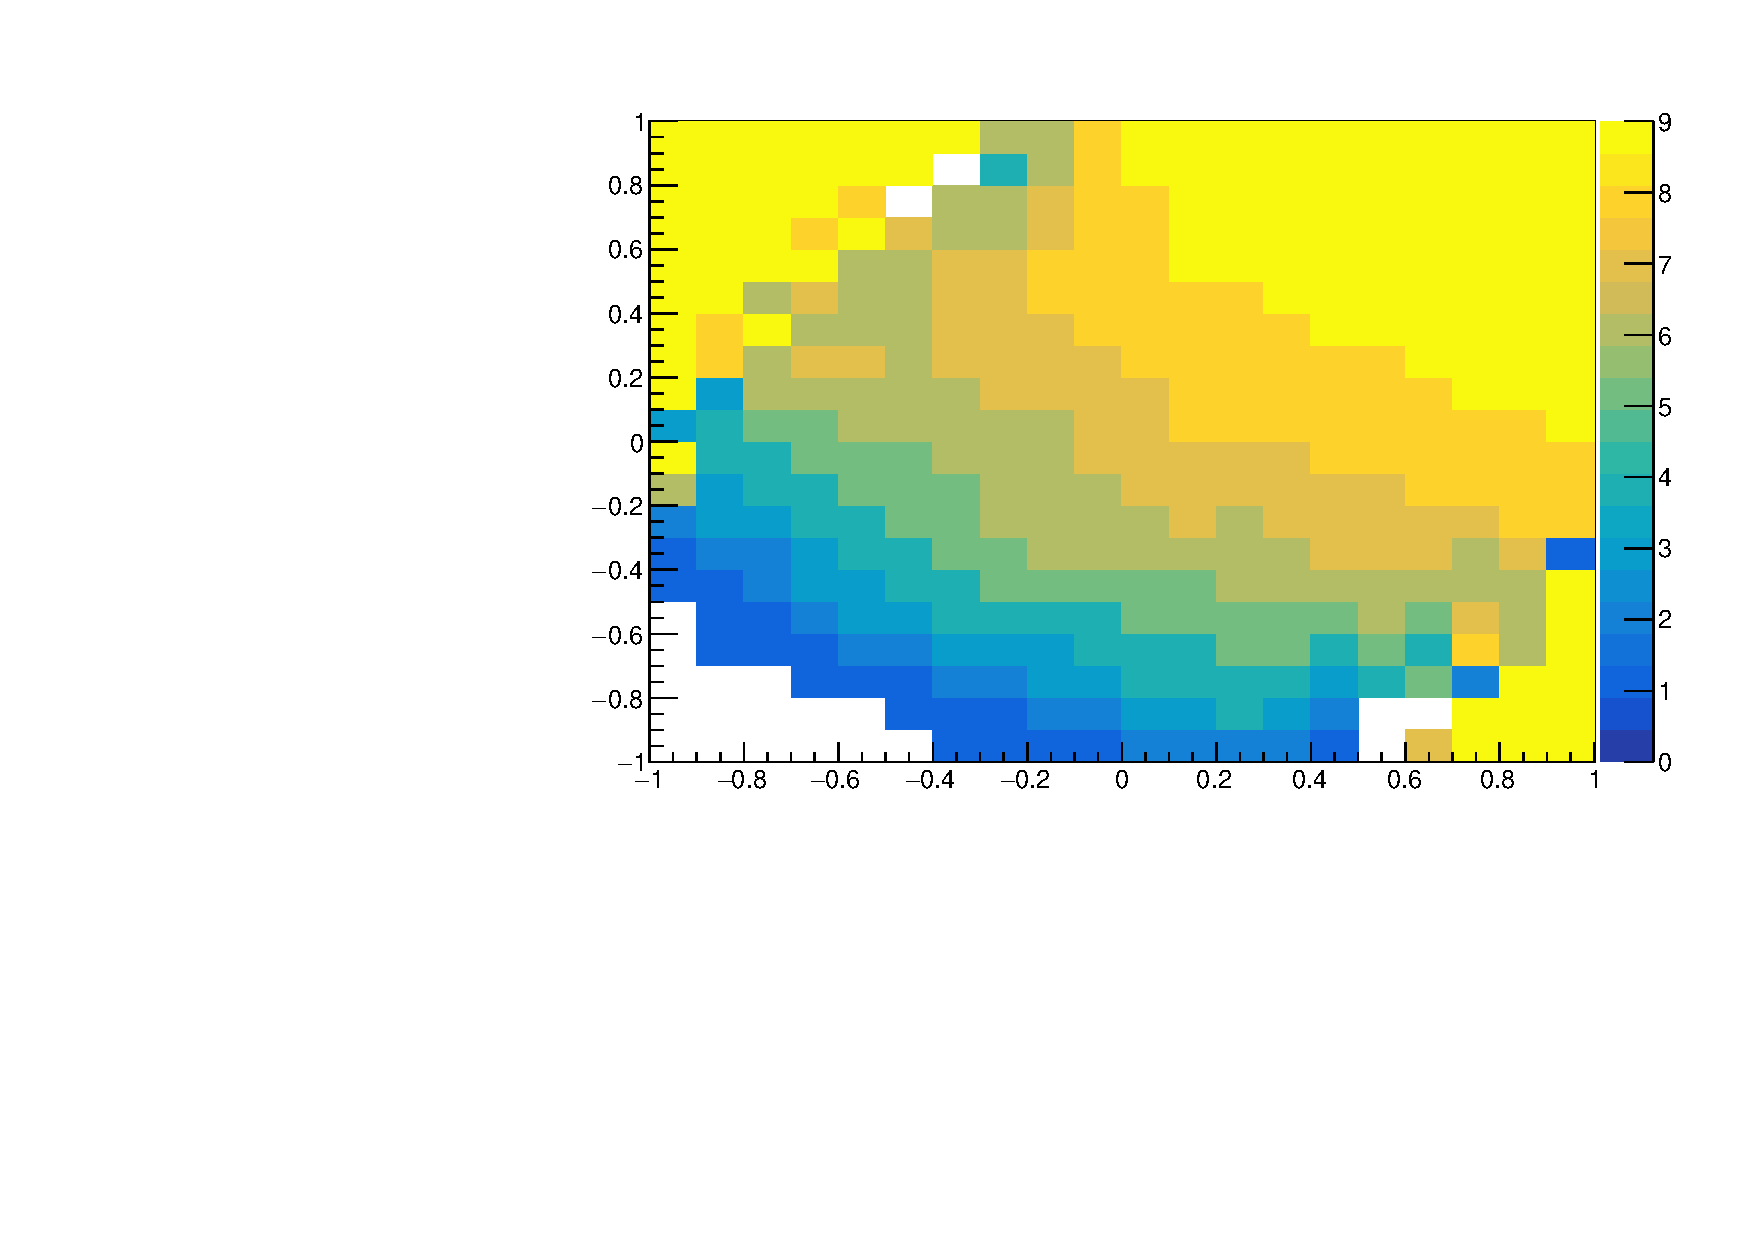
\includegraphics[width=0.45\textwidth]{binning/hTargetBinning_2lss.pdf}
  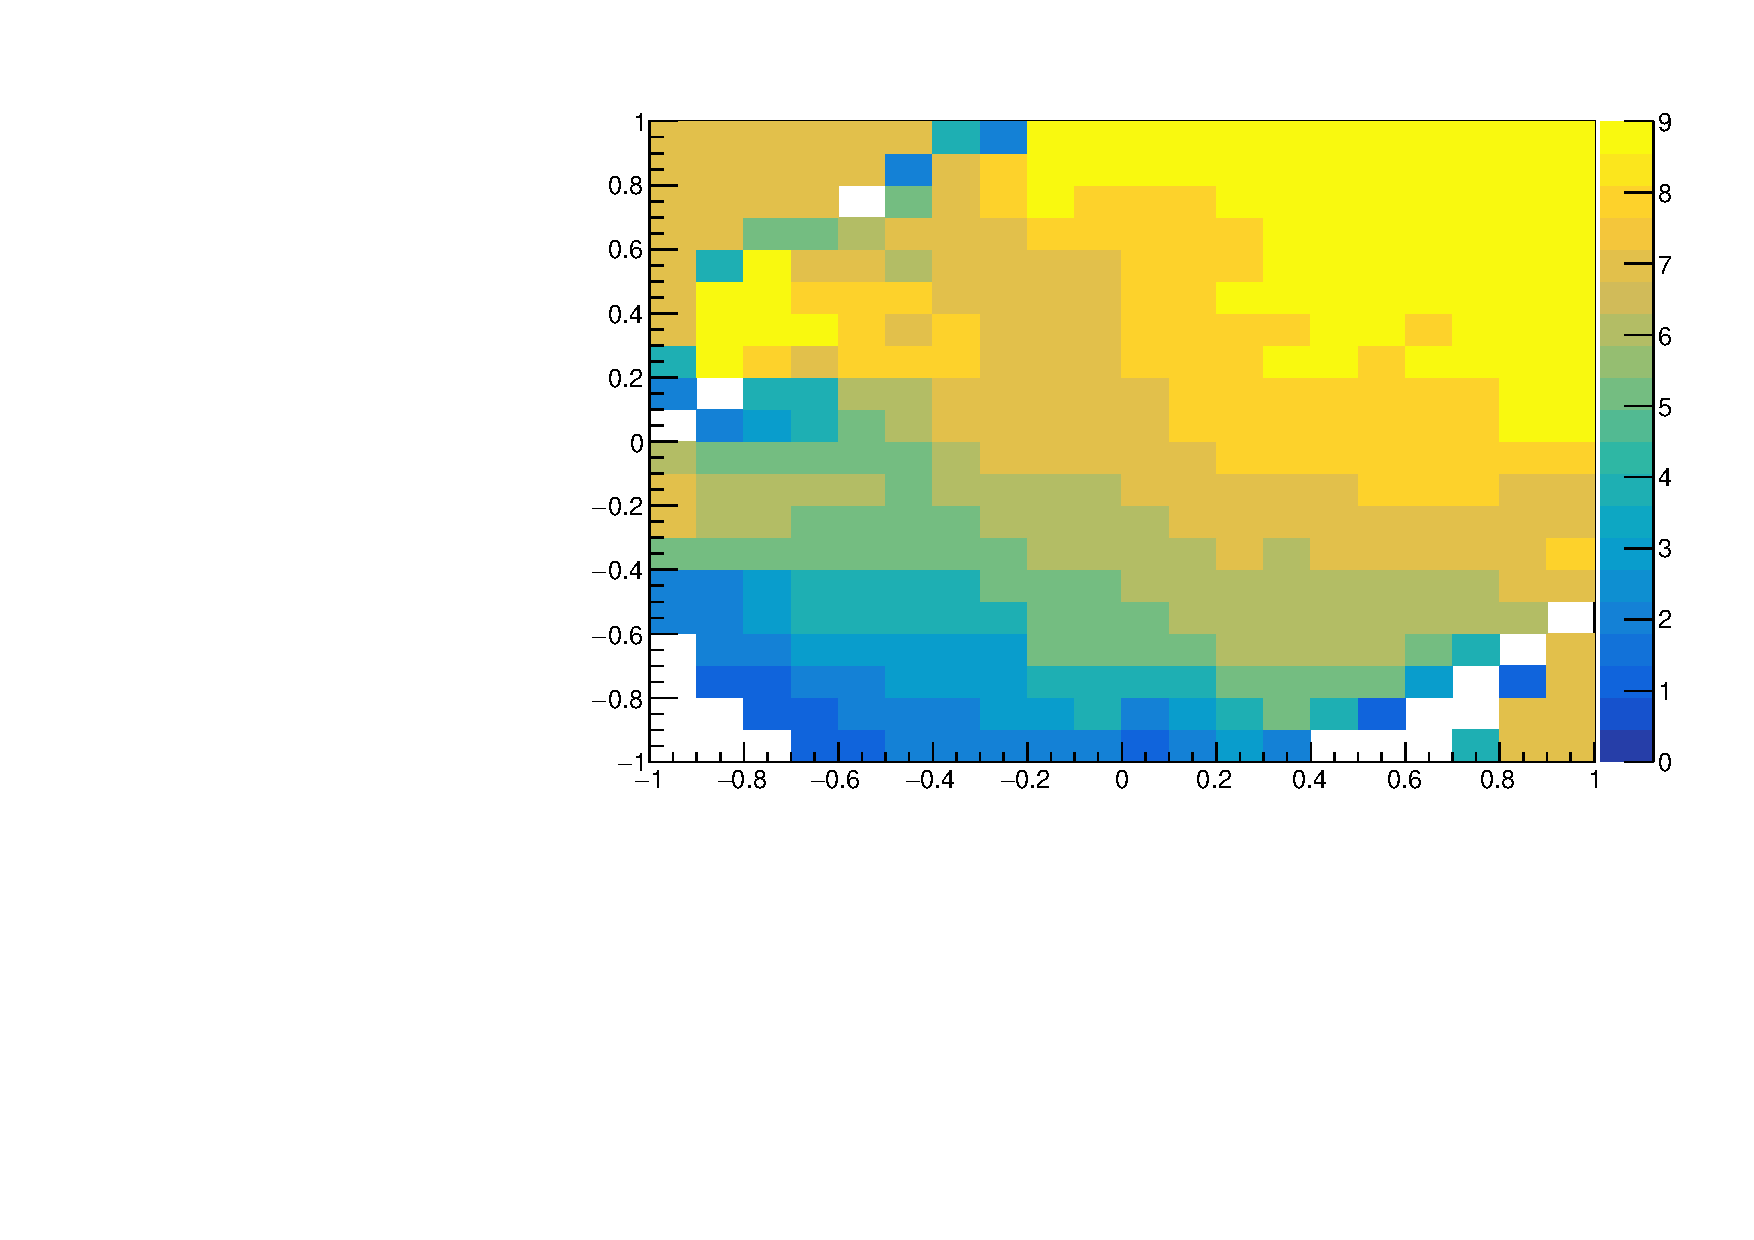
\includegraphics[width=0.45\textwidth]{binning/hTargetBinning_3l.pdf}
  \caption{Binning by S/B regions for $2lss$ (left) and $3l$ (right).}
  \label{fig:sbbinning}
\end{figure}

\begin{figure} [!h]
  \centering
  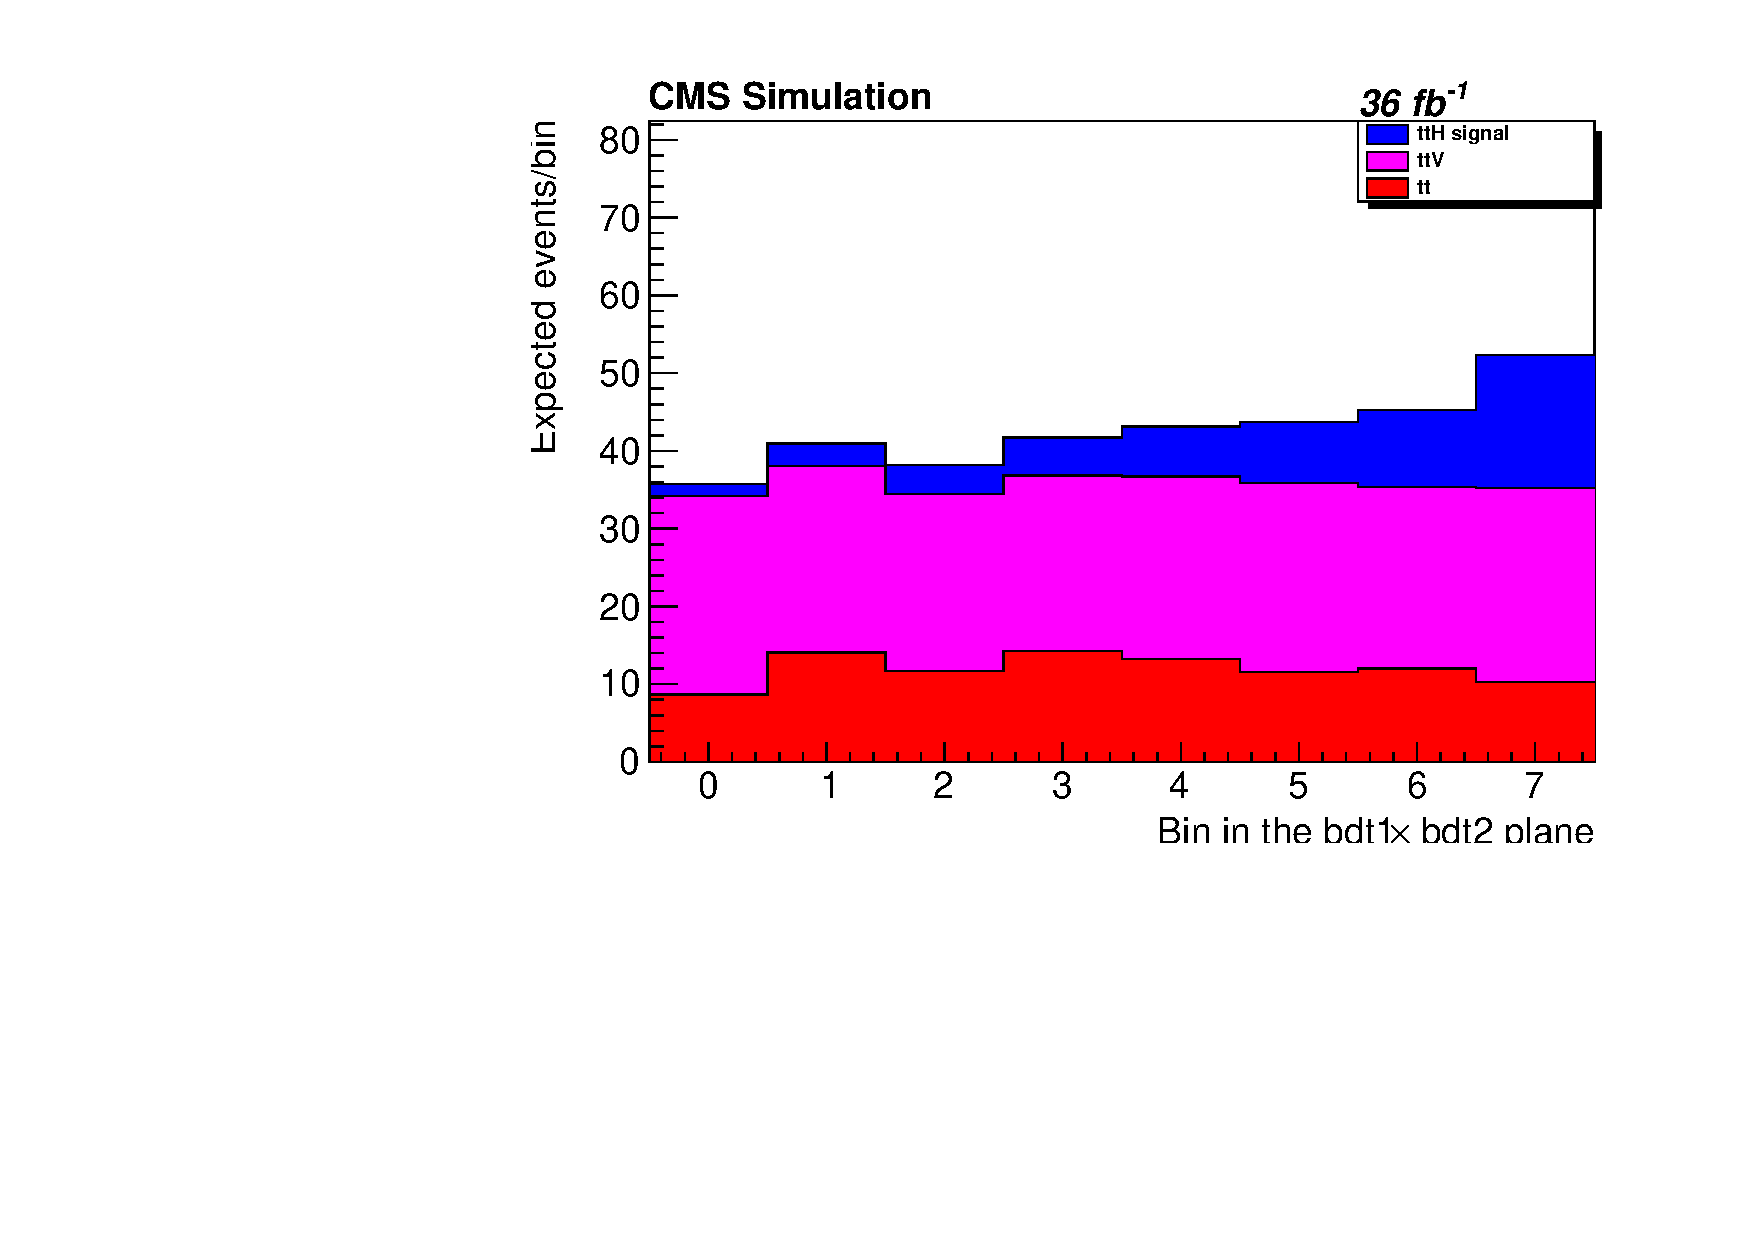
\includegraphics[width=0.45\textwidth]{binning/likelihoodBased_1d_2lss.pdf}
  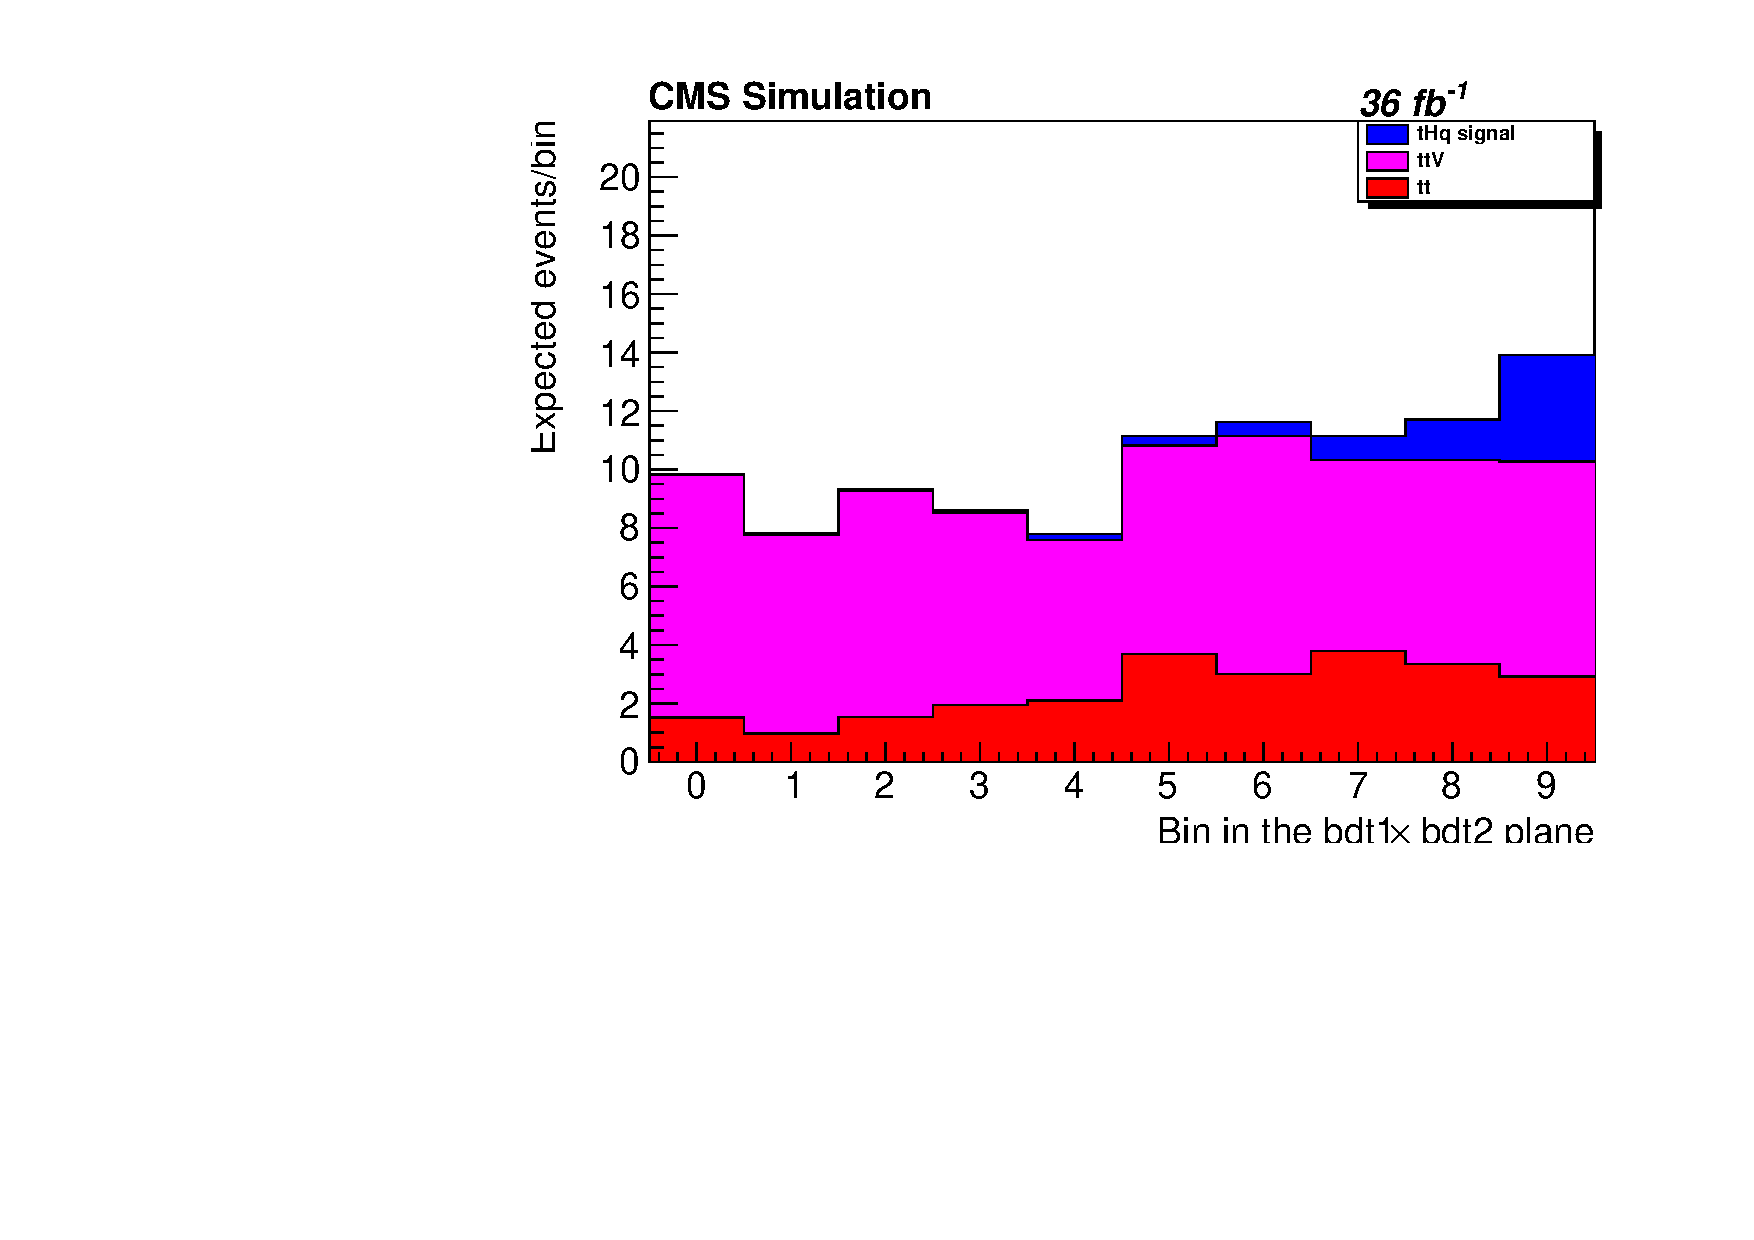
\includegraphics[width=0.45\textwidth]{binning/likelihoodBased_1d_3l.pdf}
  \caption[Final bins (corresponding to S/B regions in the 2D plane)]{Final bins (corresponding to S/B regions in the 2D plane) for $2lss$ and $3l$ (right).}
  \label{fig:sbfinalbins}
\end{figure}

Using this method, the resulting limits (for the $\Ct=-1, \CV=1$ scenario) are about 20\% worse than with the binning in Section \ref{sec:binopt}: \mumu\ changed from 1.82 to 2.15, $3l$ changed from 1.52 to 1.75.

\textbf{$k$-Means geometric clustering}\\
This method employs a recursive application of the $k$-means algorithm (see Appendix D in Reference~\cite{CMS_AN_2017-029}) to separate the 2D plane into geometric regions. The resulting clustering (using the \ttH\ multilepton code on \tHq\ signal and \ttbar\ and \ttV\ background events) are shown in Figure ~\ref{fig:kmeansbinning}. The expected distribution of events for the signal and dominant backgrounds in these bins is shown in Fig.~\ref{fig:kmeansfinalbins}.
\begin{figure} [!h]
  \centering
  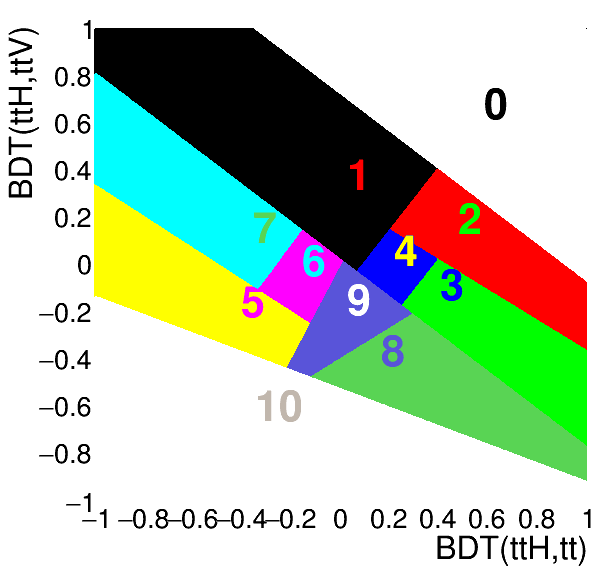
\includegraphics[width=0.45\textwidth]{binning/voronoi_2l_trial0.png}
  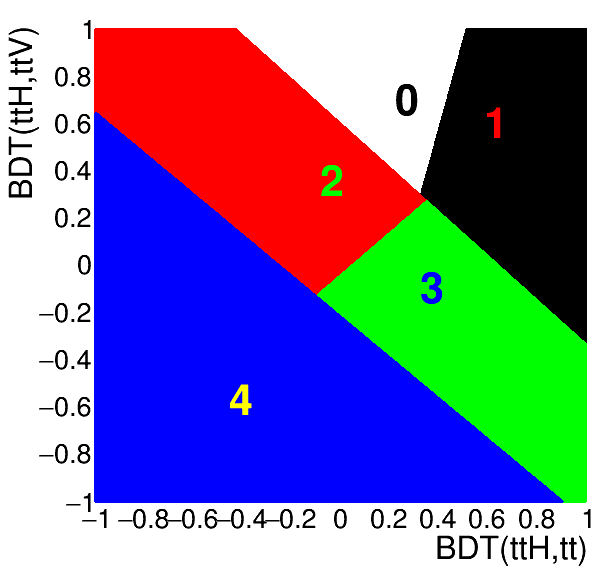
\includegraphics[width=0.45\textwidth]{binning/voronoi_3l_trial0.png}
  \caption[Binning into geometric regions using a $k$-means algorithm.]{Binning into geometric regions using a $k$-means algorithm for $2lss$ (left) and $3l$ (right).}
  \label{fig:kmeansbinning}
\end{figure}

\begin{figure} [!h]
  \centering
  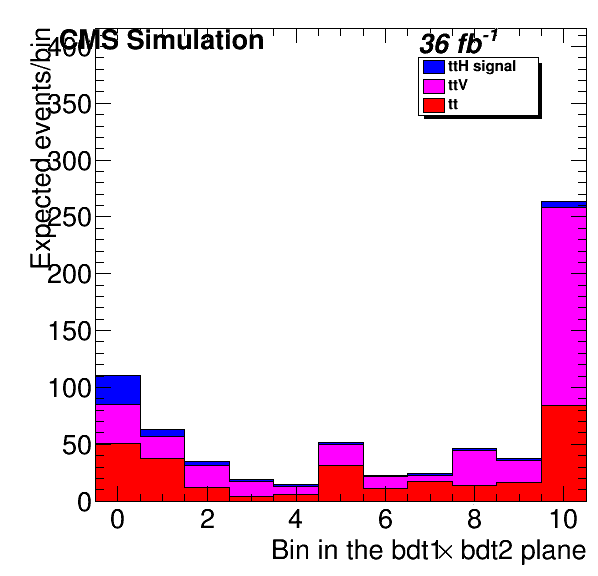
\includegraphics[width=0.45\textwidth]{binning/recursiveNoOrdering_2l_trial0.png}
  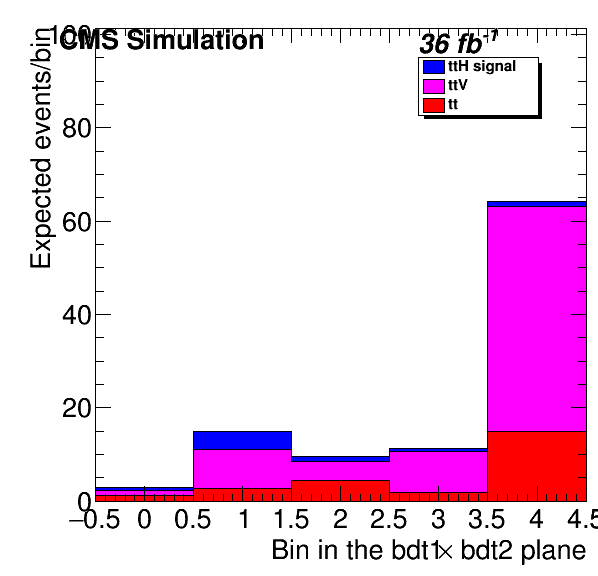
\includegraphics[width=0.45\textwidth]{binning/recursiveNoOrdering_3l_trial0.png}
  \caption[Final bins using a $k$-means algorithm.]{Final bins using a $k$-means algorithm for $2lss$ (left) and $3l$ (right). Note that the bin numbering here is such that signal-like bins are lower.}
  \label{fig:kmeansfinalbins}
\end{figure}

Similarly to the S/B ratio binning, the limits using the $k$-means clustering are significantly worse than those of the bins described before. In the \mumu\ channel, the limit deteriorates from 1.82 to 2.05, whereas in $3l$ it changes from 1.58 to 1.78.
